\documentclass[tikz,border=5pt]{standalone}
\usepackage{tikz}
\usetikzlibrary{knots,calc, hobby}

% Turn guides off when you're happy:
\newif\ifguides
\guidestrue % ← change to \guidesfalse for final

\begin{document}


%  Up Quarck knot (5_2)
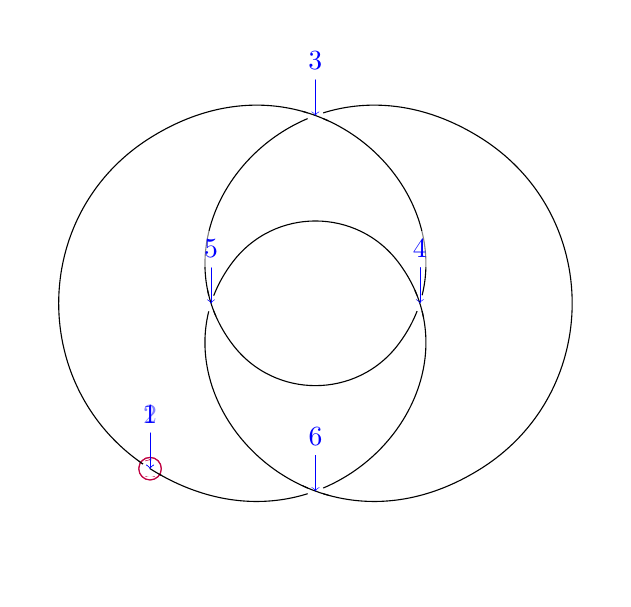
\begin{tikzpicture}[use Hobby shortcut, line cap=round, line join=round, scale=1.05]
    % ===== Up Quark knot (5_2): control points =====
\coordinate (P1) at (-2.0,  -2.0);  % start / close
\coordinate (P2) at (-2.0,  2.0);
\coordinate (P3) at ( 1, -0.5);
\coordinate (P4) at (-1, -0.5);
\coordinate (P5) at ( 2.0,  2.0);
\coordinate (P6) at ( 2.0, -2.0);
\coordinate (P7) at (-1,  0.5);
\coordinate (P8) at ( 1,  0.5);
\coordinate (P9) at (-2.0, -2.0);  % = P1 (smooth closed path)

\begin{knot}[
    consider self intersections,
    draft mode=crossings,              % show crossing indices while tuning
    ignore endpoint intersections=false,
    clip width=5pt, clip radius=3pt,
    flip crossing/.list={2,4}        % same over/under pattern as your snippet
]
\strand
([closed] P1)..(P2)..(P3)..(P4)..(P5)..(P6)..(P7)..(P8)..(P9);
\end{knot}

\ifguides
% Point labels + dashed skeleton for quick reshaping
\foreach \i/\pos in {1/above right,2/right,3/below left,4/above,5/above left,6/below,7/below right,8/left,9/above right}{
    \fill[blue] (P\i) circle (1.2pt);
    \node[blue,\pos,font=\scriptsize] at (P\i) {\i};
}
\draw[gray!40, dashed](P1)--(P2)--(P3)--(P4)--(P5)--(P6)--(P7)--(P8)--(P9);
\fi
\end{tikzpicture}





\end{document}
